\chapter{Animating the Wave Equation: Staggered Leapfrog}
\label{Lab:13}

Up to this point, we have not solved a partial differential equation.
We flirted with the idea in  chapters ~\ref{Lab:11} and \ref{Lab:12}
by using separation of variables to turn the partial differential equation into a set
of ordinary differential equations. But separating the
variables and expanding in orthogonal functions is not the only
way to solve partial differential equations, and in
many situations this technique is awkward, ineffective, or
both. Today we will study another way of solving partial
differential equations using a spatial grid and stepping
forward in time. And as an added attraction, this method
automatically supplies a beautiful animation of the solution.
We will only show you one of several algorithms of this type
that can be used on wave equations, so this is just an
introduction to a larger subject. \index{Staggered
leapfrog!wave equation} \index{Wave equation!via staggered
leapfrog} The method we will show you here is called {\it
staggered leapfrog}; it is the simplest good method that we
know.

\labsection{The wave equation with staggered leapfrog}

Consider again the classical wave equation with wave speed $c$.
(For instance, for waves on a string $c=\sqrt{T/ \mu}$.)
\index{Wave equation!boundary conditions}
\index{Boundary conditions!Dirichlet}
\index{Dirichlet boundary conditions}
\begin{equation}
    {\partial^2 y \over \partial t^2} - c^2 {\partial^2 y \over \partial x^2} = 0
\end{equation}
The boundary conditions to be applied are usually either of {\it
Dirichlet} type (values specified):
\index{Boundary conditions!Neumann}
\index{Neumann boundary conditions}
\begin{equation}
    y(0,t)=f_\mathrm{left}(t)~~~;~~~y(L,t)=f_\mathrm{right}(t)
\end{equation}
or of {\it Neumann} type (derivatives specified):
\begin{equation}
    {\partial y \over \partial x}(0)=g_\mathrm{left}(t)~~~;~~~
    {\partial y \over \partial x}(L)=g_\mathrm{right}(t)
\end{equation}
Some mixed boundary conditions specify a relation between the value
and derivative (as at the bottom of the hanging chain). These
conditions tell us what is happening at the ends of the string. For
example, maybe the ends are pinned
($f_\mathrm{left}(t)=f_\mathrm{right}(t)=0$); perhaps the ends slide
up and down on frictionless rings attached to frictionless rods
($g_\mathrm{left}(t)=g_\mathrm{right}(t)=0$); or perhaps the left end
is fixed and someone is wiggling the right end up and down
sinusoidally ($f_\mathrm{left}(t)=0$ and $f_\mathrm{right}(t)=A
\sin{\omega t}$). In any case, some set of conditions at the ends are
required to be able to solve the wave equation.

\index{Initial conditions!wave equation}
\index{Wave equation!initial conditions}
It is also necessary to specify the initial state of the string,
giving its starting position and velocity as a function of position:
\begin{equation}\label{eq:WaveIC}
    y(x,t=0) = y_0(x)~~~~;~~~~{\partial y(x,t) \over \partial t} |_{t=0}    = v_0(x)
\end{equation}
\marginfig[1.5in]{Figures/f05p3a}{Snapshots of the evolution of a wave on a
string with fixed ends and an initial displacement but no
initial velocity. (See Problem~\ref{P:13.3a})}  

Both of these initial conditions are necessary because the wave
equation is second order in time, just like Newton's second law, so
initial displacements and velocities must be specified to find a
unique solution.

To numerically solve the classical wave equation via staggered
leapfrog we approximate both the time and spatial derivatives with
centered finite differences. In the notation below spatial position
is indicated by a subscript $j$, referring to grid points $x_j$,
while position in time is indicated by superscripts $n$, referring
to time steps $t_n$ so that $y(x_j,t_n)=y_j^n$. The time steps and
the grid spacings are assumed to be uniform with time step called
$\tau$ and grid spacing called $h$.
\begin{equation}\label{eq:TimeDeriv}
    \frac{\partial^2 y}{\partial t^2} \approx
    \frac{y_j^{n+1} - 2 y_j^n + y_j^{n-1}}{\tau^2}
\end{equation}
\begin{equation}\label{eq:SpaceDeriv}
\frac{\partial^2 y }{\partial x^2} \approx
\frac{y^n_{j+1} - 2 y^n_{j} +  y^n_{j-1}}
{h^2}
\end{equation}



The staggered leapfrog algorithm is simply a way of finding
$y_j^{n+1}$ ($y_j$ one time step into the future) from the current
and previous values of $y_j$. To derive the algorithm just put these
two approximations into the classical wave equation and solve for
$y_j^{n+1}$: \footnote{N.\ Asmar, {\it Partial Differential
Equations and Boundary Value Problems} (Prentice Hall, New Jersey,
2000), p. 421-429.}
\begin{equation}
    y_j^{n+1} = 2 y_j^n - y_j^{n-1} + {c^2 \tau^2 \over h^2}
    \left( y^n_{j+1} - 2 y^n_{j} +  y^n_{j-1}
    \right)
    \label{leapfrog}
\end{equation}

\begin{enumerate}
\probtwo \label{P:13.1} Derive Eq.~\eqref{leapfrog} from the
approximate second derivative formulas. (You can use
mathematica if you like, but this is really simple to do by
hand.)
\end{enumerate}

Equation~\eqref{leapfrog} can only be used at interior spatial
grid points because the $j+1$ or $j-1$ indices reach beyond the
grid at the first and last grid points. The behavior of the
solution at these two end points is determined by the boundary
conditions. Since we will want to use both fixed value
(Dirichlet) and derivative (Neumann) boundary conditions, let's
use a \textbf{cell-centered grid with ghost points} (with $N$ cells and
$N+2$ grid points) so we can easily handle both types without
changing our grid. \index{Dirichlet boundary conditions} If the
values at the ends are specified (Dirichlet boundary
conditions) we have
\begin{equation}
    {y_1^{n+1}+y_2^{n+1} \over 2} = f_\mathrm{left}(t_{n+1})~~~\Rightarrow~~~
    y_1^{n+1}=-y_2^{n+1} + 2 f_\mathrm{left}(t_{n+1})
    \label{bdyfirst}
\end{equation}
\begin{equation}
    {y_{N+2}^{n+1}+y_{N+1}^{n+1} \over 2} = f_\mathrm{right}(t_{n+1})~~~\Rightarrow~~~
    y_{N+2}^{n+1}=-y_{N+1}^{n+1} + 2 f_\mathrm{right}(t_{n+1})
\end{equation}
\index{Neumann boundary conditions} If the derivatives are
specified (Neumann boundary conditions) then we have
\begin{equation}
    {y_2^{n+1}-y_1^{n+1} \over h} = g_\mathrm{left}(t_{n+1})~~~\Rightarrow~~~
    y_1^{n+1}=y_2^{n+1} - h g_\mathrm{left}(t_{n+1})
\end{equation}
\begin{equation}
    {y_{N+2}^{n+1}-y_{N+1}^{n+1} \over h} = g_\mathrm{right}(t_{n+1})~~~\Rightarrow~~~
    y_{N+2}^{n+1}=y_{N+1}^{n+1} + h g_\mathrm{right}(t_{n+1})
    \label{bdylast}
\end{equation}
To use staggered leapfrog, follow the following steps:

\begin{enumerate}
\item Advance the solution at all
interior points to the next time step using
Eq.~(\ref{leapfrog})
\item Apply the boundary conditions
using the appropriate equation from
Eqs.~(\ref{bdyfirst})-(\ref{bdylast}) to find the values of $y$
at the end points
\item Repeat to take another step forward in time.
\end{enumerate}

\index{Initial conditions!wave equation}
\marginfig[-1in]{Figures/f05p3b}{Snapshots of the evolution of a wave on a string with
free ends and an initial displacement but no initial velocity.
(See Problem~\ref{P:13.3b})}
The staggered leapfrog algorithm in Eq.~(\ref{leapfrog})
requires not just $y$ at the current time level $y_j^n$ but
also $y$ at the previous time level $y_j^{n-1}$. This means
that we'll need to keep track of three arrays: an array {\tt y}
for the current values $y_j^{n}$, an array {\tt yold} for the
values at the previous time step $y_j^{n-1}$, and an array {\tt
ynew} for the values at the next time step $y_j^{n+1}$. At time
$t=0$ when the calculation starts, the initial position
condition gives us the current values $y_j^{n}$, but we'll have
to make creative use of the initial velocity condition to
create an appropriate {\tt yold} to get started. To see how
this works, let's denote the initial values of $y$ on the grid
by $y_j^0$, the values after the first time step by $y_j^1$,
and the unknown previous values ({\tt yold}) by $y_j^{-1}$. A
centered time derivative at $t=0$ turns the initial velocity
condition from Eq.~\eqref{eq:WaveIC} into
\begin{equation}\label{eq:leapfrogIV}
    {y_j^1-y_j^{-1} \over 2 \tau} = v_0(x_j)
\end{equation}
This gives us an equation for the previous values $y_j^{-1}$,
but it is in terms of the still unknown future values
$y_j^{1}$. However, we can use Eq.~\eqref{leapfrog} to obtain
another relation between $y_j^1$ and $y_j^{-1}$. Leapfrog at
the first step ($n=0$) says that
\begin{equation}
    y_j^{1} = 2 y_j^0 - y_j^{-1} + {c^2 \tau^2 \over h^2}
    \left( y^0_{j+1} - 2 y^0_{j} +  y^0_{j-1}
    \right)
    \label{leapfrog0}
\end{equation}
If we insert this expression for $y_j^1$ into
Eq.~\eqref{eq:leapfrogIV}, we can solve for $y_j^{-1}$ in terms of
known quantities:
\begin{equation}\label{eq:yold}
    y_j^{-1}=y_j^0-v_0(x_j) \tau +
    {c^2 \tau^2 \over 2 h^2}
    \left( y^0_{j+1} - 2 y^0_{j} +  y^0_{j-1} \right)
\end{equation}

\begin{enumerate}
\probtwo \label{P:13.2} Derive Eq.~\eqref{eq:yold} from
Eqs.~\eqref{eq:leapfrogIV} and \eqref{leapfrog0}.
\end{enumerate}

Now we have all the pieces we need to start coding.



\clearpage




\marginfig[-0.3in]{Figures/f05p3c}{Snapshots of the evolution of a wave on a
string with fixed ends and no initial displacement but with an
initial velocity. (See Problem~\ref{P:13.3c})} 

\begin{enumerate}
\probtwo \label{P:13.3} Consider the motion of a guitar string, fixed
at both ends:
\[
    y(0) = 0 \quad ; \quad y(L) = 0
\]
The string is plucked so that the initial waveform is given by:
\[
y(x,0) = e^{-\frac{160 (x - {L \over 2})^2}{L^2}} - e^{-\frac{160 {L\over 2}^2}{L^2} }
\]
\begin{enumerate}
  \subprob \label{P:13.3a} Run an animation of the guitar string long
  enough that you can see the reflection from the ends and the way the
  two pulses add together and pass right through each other.  

  \subprob Start experimenting with the time step ($\tau$). Show by
  numerical experimentation that if $\tau>h/c$ the algorithm blows up
  spectacularly.  \index{Instability, numerical} \index{Numerical
    instability} \index{CFL condition} \index{Courant condition} This
  failure is called a {\it numerical instability} and we will be
  trying to avoid it all semester. This limit is called the {\it
    Courant-Friedrichs-Lewy condition}, or sometimes the {\it CFL
    condition}, or sometimes (unfairly) just the {\it Courant
    condition}.  

  \subprob \label{P:13.3b} Now change the boundary conditions so that
  ${\partial y \over \partial x}=0$ at each end and watch how the
  reflection occurs in this case.  

\subprob \label{P:13.3c} Now change the initial
  conditions from initial displacement with zero velocity to initial
  velocity with zero displacement. Use an initial Gaussian velocity
  pulse just like the displacement pulse you used earlier and use
  fixed-end boundary conditions. Watch how the wave motion develops in
  this case. Then find a slinky, stretch it out, and whack it in the
  middle to verify that the math does the physics right.
\end{enumerate}
\end{enumerate}
\ifsolutions
\textit{Solution:}\\
\begin{codeexample}
\begin{VerbatimOut}{\listingFile}

class animatedWave():

    def __init__(self,a,b,c,N,tau,tMax,stabilityCheck = False):
        from numpy import arange
        self.L = b
        self.c = c
        self.N = N
        self.tMax = tMax
        self.tau = tau
        self.dx = (b - a)/N
        self.x = arange(a - self.dx/2., b + self.dx,self.dx)
        
        if self.tau > self.dx/self.c and stabilityCheck:
            print 'Beware: your algorithm will be unstable.'
            import sys
            sys.exit()


    def initializeWave(self):
        from numpy import exp,zeros
        # Gaussian initial displacement
        self.y = exp( -160/self.L**2 * (self.x - self.L/2.)**2 ) - exp( -160/self.L**2 * (0 - self.L/2.)**2 )
        # Zero initial velocity
        self.v = zeros(self.N+2)


    def animate(self):
        from numpy import zeros_like,copy
        from matplotlib import pyplot
        constant = self.c**2 * self.tau**2/(2 * self.dx**2)

        yOld = zeros_like(self.y)
        yOld[1:self.N + 1] = self.y[1:self.N+1] - self.v[1:self.N + 1] * self.tau + constant * (self.y[2:self.N + 2] - 2 * self.y[1:self.N + 1] + self.y[0:self.N])
        yOld[0] = yOld[1]
        yOld[-1] = yOld[-2]
        t = 0
        counter = 0
        while t < self.tMax:
            yNew = zeros_like(self.y)
            yNew[1:self.N + 1] = 2 * self.y[1:self.N+1] - yOld[1:self.N + 1] + constant * ( self.y[2:self.N + 2] - 2 * self.y[1:self.N + 1] + self.y[0:self.N])
            yNew[0] =  yNew[1]
            yNew[-1] =  yNew[-2]

            if counter % 20 == 0:
                pyplot.plot(self.x,self.y,'r.-')
                pyplot.ylim(-1,1)
                pyplot.draw()
                pyplot.pause(.000001)
                pyplot.clf()


            yOld = copy(self.y)
            self.y = copy(yNew)


            t += self.tau
            counter += 1
a = 0
b = 1.
c = 2.
N = 200
tau = 0.001
tMax = 10
myWave = animatedWave(a,b,c,N,tau,tMax,stabilityCheck = True)
myWave.initializeWave()
myWave.animate()
\end{VerbatimOut}
\end{codeexample}
\else
\noindent\rule{5 in}{0.01 in}
\fi

\medskip

\begin{figure}[b]
\centerline{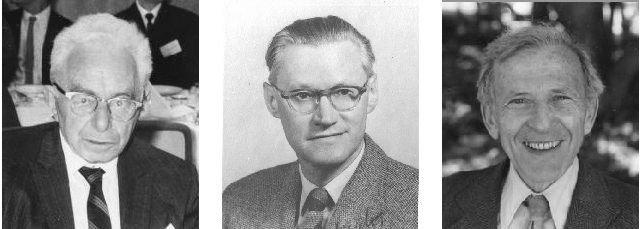
\includegraphics{Figures/f05Courant}}
\caption{Richard Courant (left), Kurt Friedrichs
(center), and  Hans Lewy (right) described the CFL
instability condition in 1928.}
\end{figure}


\labsection{Homework}
\begin{enumerate}
\prob Modify your leapfrog program to use $T = 1$ N and $\mu(x) = 0.1 +
{x\over L}$ so that the linear mass density of the guitar string
increases toward the right. (This makes the wave speed be a function of position, $c=c(x)$.)
Watch how the pulses propagate and explain qualitatively why they behave
as they do.
\end{enumerate}
\ifsolutions
\textit{Solution:}\\
\begin{codeexample}
\begin{VerbatimOut}{\listingFile}

class animatedWave():

    def __init__(self,a,b,N,tau,tMax,stabilityCheck = False,variableMu = False, T = 1, c = 2):
        from numpy import arange
        self.L = b        
        self.N = N
        self.tMax = tMax
        self.tau = tau
        self.dx = (b - a)/N
        self.x = arange(a - self.dx/2., b + self.dx,self.dx)

        if variableMu:
            from numpy import sqrt, array
            self.c = sqrt(T/array([self.mu(var) for var in self.x]))
        else: 
            self.c = c

        print stabilityCheck, 'here'
        from numpy import any
        if any(self.tau > self.dx/self.c) and stabilityCheck:
            print 'Beware: your algorithm will be unstable.'
            import sys
            sys.exit()


    def initializeWave(self):
        from numpy import exp,zeros
        # Gaussian initial displacement
        self.y = exp( -160/self.L**2 * (self.x - self.L/2.)**2 ) - exp( -160/self.L**2 * (0 - self.L/2.)**2 )
        # Zero initial velocity
        self.v = zeros(self.N+2)

    def mu(self,x):
        return 0.1 + x/self.L

    def animate(self):
        from numpy import zeros_like,copy
        from matplotlib import pyplot
        constant = self.c**2 * self.tau**2/(2 * self.dx**2)

        yOld = zeros_like(self.y)
        yOld[1:self.N + 1] = self.y[1:self.N+1] - self.v[1:self.N + 1] * self.tau + constant[1:self.N + 1] * (self.y[2:self.N + 2] - 2 * self.y[1:self.N + 1] + self.y[0:self.N])
        yOld[0] = -yOld[1]
        yOld[-1] = -yOld[-2]
        t = 0
        counter = 0
        while t < self.tMax:
            yNew = zeros_like(self.y)
            yNew[1:self.N + 1] = 2 * self.y[1:self.N+1] - yOld[1:self.N + 1] + constant[1:self.N + 1] * ( self.y[2:self.N + 2] - 2 * self.y[1:self.N + 1] + self.y[0:self.N])
            yNew[0] =  -yNew[1]
            yNew[-1] = - yNew[-2]

            if counter % 50 == 0:
                pyplot.plot(self.x,self.y,'r.-')
                pyplot.ylim(-1,1)
                pyplot.draw()
                pyplot.pause(.000001)
                pyplot.clf()


            yOld = copy(self.y)
            self.y = copy(yNew)


            t += self.tau
            counter += 1
a = 0
b = 1.
c = 2.
N = 200
tau = 0.001
tMax = 10

myWave = animatedWave(a,b,N,tau,tMax,stabilityCheck = True, variableMu = True)
myWave.initializeWave()
myWave.animate()
\end{VerbatimOut}
\end{codeexample}
\else
\noindent\rule{5 in}{0.01 in}
\fi




